\documentclass{article}
\setcounter{secnumdepth}{-1}
\usepackage{graphicx}
\usepackage{hyperref}
\usepackage{amsfonts}
\usepackage{amsmath}
\usepackage{cite}
\usepackage[margin=0.9in, paperwidth=8.5in, paperheight=11in]{geometry}
\begin{document}
\title{S.I.E.V.E. Progress Report}
\author{Graham Clenaghan \\ Nick Kullman \\ Wayne Yang}
\date{Spring 2015}
\maketitle

\section{Sieve Analysis for Vaccine Trials}

Sieve analysis is a statistical tool that aims to improve vaccine efficacy by providing information regarding how vaccine efficacy depends on characteristics of an exposing pathogen. 
Since the mid 1990s, it has been used in vaccine trials for cholera, HIV-1, hepatitis B, rotavirus, and pneumococcus. 
The metaphorical ``sieve'' in sieve analysis is the vaccine's genomic / proteomic sequence-specific immunity barrier to disease. The pathogen penetrates the vaccine's immunity barrier through ``holes'' in the ``sieve'' to cause disease \cite{gilbert2001sieve}.
Determining which characteristics of the pathogen's genomic / proteomic sequence allow it to pass through the holes will suggest antigens to include in future vaccine constructions to fight the pathogen.
Determining these characteristics is the purpose of sieve analysis. 
\\
Our project aims to help vaccine researchers explore data from trials and and aid in performing sieve analysis of the results, which involves a comparison of the genomes of strains infecting patients administered a vaccine and patients administered a placebo.

While there are some existing visualizations, none of them completely fulfill this task and do not allow easy manipulation of the graphic and exploration of the data at the level we hope to accomplish. We also aim to make the tool extensible and the final product polished enough to be used by researchers in the field for use in publications in further vaccine studies.

\section{Sequence Data Visualization Tools}

There are several existing tools for the visualization of genomic / proteomic sequence data.  Some of these tools tend to provide a very detailed display of the alignments of sequences for a particular gene / protein from multiple patients.  While this approach allows a user to see all of their data at once, it does not provide quick and easy analysis of particular sites in the sequence across patients or subsets of patients.  The following example is from a software called Aliview \cite{aliview}.

\begin{center}
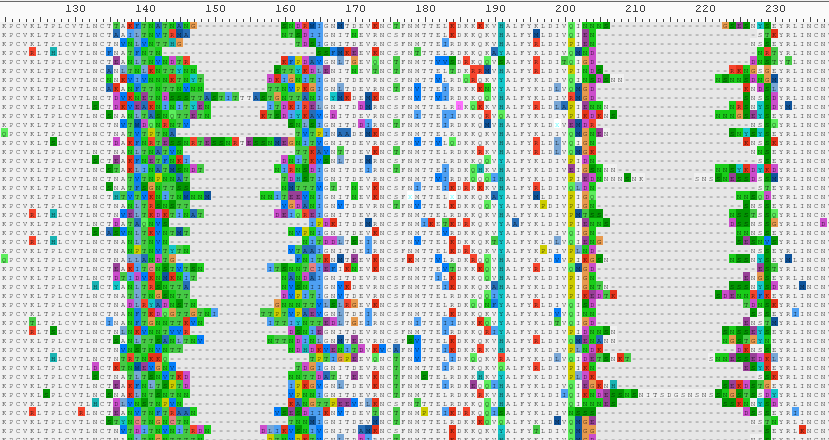
\includegraphics[height=3in,width=4in]{aliview.png}
\end{center}
Clearly, understanding the pattern of mutations and any relationships to treatment status for a particular site in the sequence is very difficult to do in this view with any precision.
\\
\newline
\noindent Other tools are geared towards specific analyses of sequence data.  The following figure was generated using WebLogo \cite{weblogo}, which is an online tool that can be used to parse sequence data and generate plots:
\begin{center}
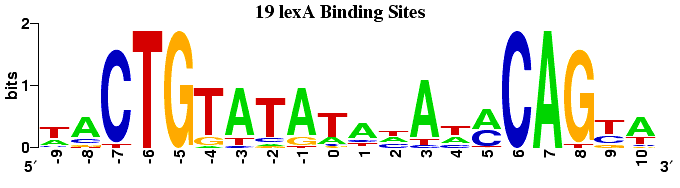
\includegraphics[height=1in,width=4in]{lexA.png}
\end{center}
Ignoring some of the aesthetic choices, the main issue is that the primary user interface looks like this:
\begin{center}
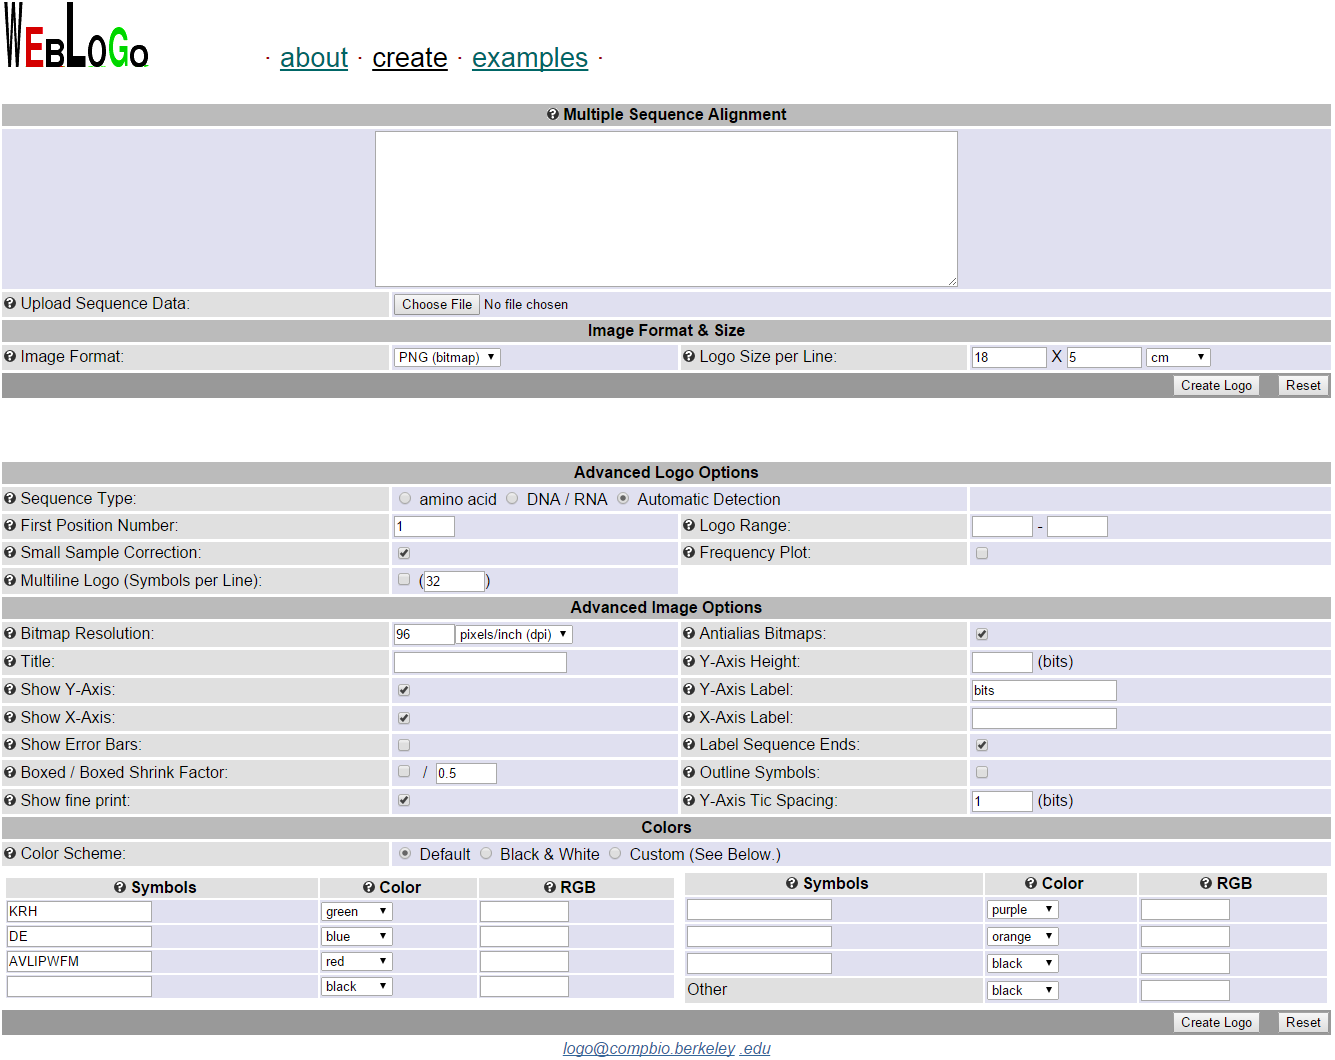
\includegraphics[height=3in,width=4in]{webloginterface.png}
\end{center}
While a graphic can be automatically generated, the user has to be quite specific about what is actually plotted.  As a result, if there are some sites that are known to be interesting, then a researcher can use WebLogo to construct plots.  However, this system makes exploratory data analysis and actually browsing the visualization rather difficult.
\\
\newline
\noindent Another tool that came up in our discussions with Dr. Gartland is the HIV Genome Browser, which allows users to browse reference data hosted online \cite{hivgenomebrowser}.   The browser is highly interactive and allows a user to explore the available sequences.   However, this visualization does not easily allow a user to import their own data and compare across patients and treatment groups as required by sieve analysis.  

The main inspiration for the project is from the paper \cite{edlefsen2014comprehensive}, which performs sieve analysis on an HIV vaccine trial. Graphics generated in this paper include an overview of the HIV genome with statistically significant sites annotated:
\begin{center}
	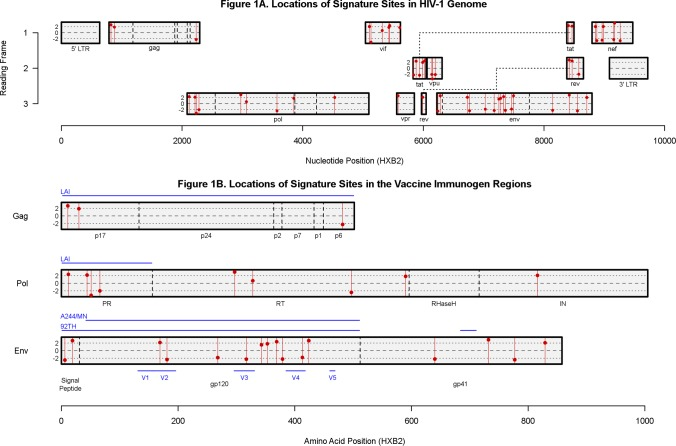
\includegraphics[width=7in]{fig2}
\end{center}
and charts of individual sites showing mismatch prevalence.
\begin{center}
	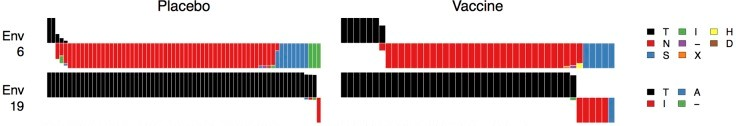
\includegraphics[width=7in]{fig3}
\end{center}
These graphics were generated by a python script which requires manual coding to generate each plot. We hope to improve on this by creating an interactive tool to aid in graphic generation and aid in exploring the data visually.


\section{Project Plan}

A work-in-progress prototype is available here: \url{http://cse512-15s.github.io/fp-nkullman-gclenagh-wfyang/}.
The utility currently supports a very basic selection mechanism of amino acid sites, which generates charts showing the prevalence of mismatches between the HIV strains found in patients and those found in the vaccine itself, and a chart showing the distribution of distances from the vaccine to the patient strains. These charts form the basic analysis tools for sieve analysis, which has the hypothesis that the strains which patients are infected with will differ between the vaccine and placebo groups at statistically significant rates.\\

The remaining tasks are roughly:
\begin{itemize}
\item Finalize the site selection mechanism / interface.  Primary member: Nick.
\item Color palette selection menu.  Primary member: Graham.
\item Incorporate p-values / entropy calculations. Primary member: Wayne.
\item Enable exporting of graphics. 
\item General polish / optimizations. 
\end{itemize}

\bibliographystyle{unsrt}
\bibliography{progress}

\end{document}
